\chapter{Background}

  \section{Neural Networks}

    Neural Networks (NNs) are key components in Artificial Intelligence (AI) and Deep Learning.
    They try to simulate some properties and the functionality of biological neural networks, like our brain, by imitating the way biological neural systems process data.
    Today, they have been applied successfully to speech recognition, face recognition on images or the transformation from speech to text.
    They are used to model software agents in video games, let autonomous robots learn new things or find patterns in data.

    A neural network consists of multiple layers.
    An input layer, one or many more hidden layers and an output layer.
    Each of these layers contain multiple neurons.

    % \begin{figure}
    %     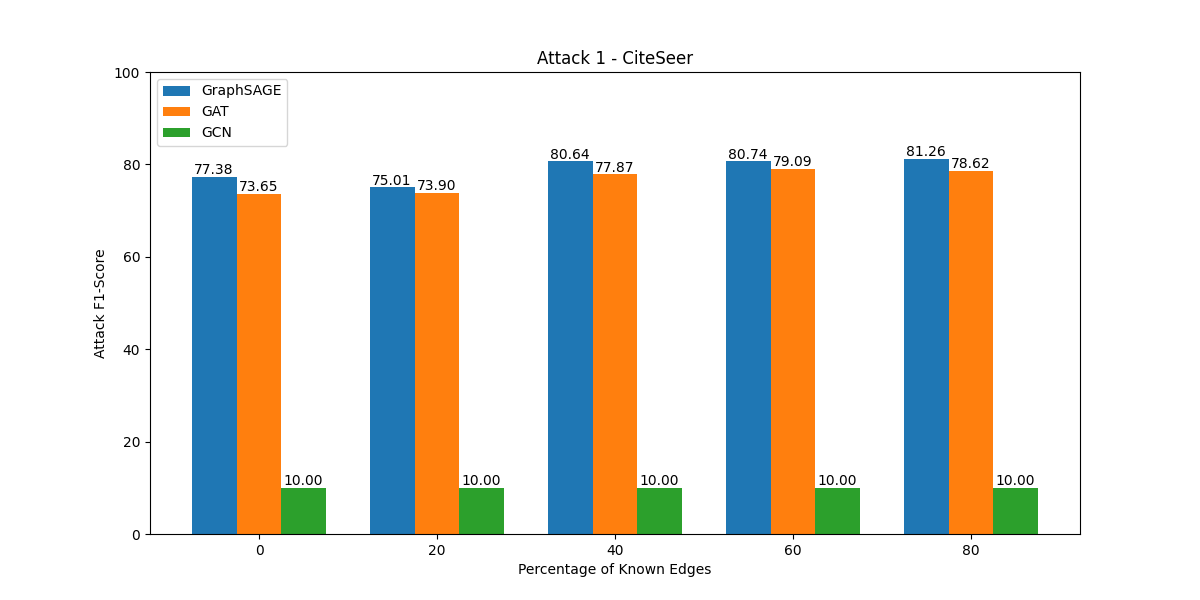
\includegraphics[scale=0.5]{res/Figures/attack-1-citeseer}
    %     \caption{This is an attacker}
    %     This is something else
    % \end{figure}

	\section{Graphs}

		As Graph we denote a data structure that contains nodes and edges. A node can have multiple attributes describing it and an edge describes the relationship between them. The most popular example where graphs are used, are social networks. The nodes represent the users that have multiple attributes like location, gender, work place etc. In a directed graph user $A$ will have an outgoing edge and user $B$ an ingoing edge if $A$ follows $B$ and vice versa. In an undirected graph the edge won't have a direction. Which means that either $A$ follows $B$, $B$ follows $A$ or both will lead to the same result, namely only one edge that is drawn, describing their relationship to each other.

	\section{Graph Neural Networks}
      
    % Describe how to query a graph neural network (f(Graph, node))

    \subsection{Transductive Learning}

    \subsection{Inductive Learning}
